\chapter{文獻回顧}
\fontsize{12pt}{18pt}\selectfont %字體大小,行距

% ------------------------- 2.0 ------------------------- %
本論文研究主題為評估個人化模型之肌肉參數,在文獻回顧中,首先會介紹關於人體動作量測的技術,
包含動作捕捉系統、感測裝置等介紹,接續會討論關於動作模擬與分析的部分,主要切割為三部分,
前半部將先引入人體模擬流程與系統介紹,並依照複雜程度進行模型分類,後半部則是關於人體的模擬與分析資訊,
最後則會回顧個人化模型的相關文獻,統整現今學者在肌肉參數領域的研究,其針對不同方法來進行介紹,
例如以直接量測或是間接估測來取得肌肉參數。第二章節將圍繞在該研究主題的背景與現況來進行探討,最終闡述肌肉參數的重要性。

% ------------------------- 2.1 ------------------------- %
\section{動作捕捉系統}
% 概述人體動作捕捉,再說分為單感測器動作捕捉系統及多感測器動作捕捉系統,單感測動作捕捉系統又分為光學動作系統及無學動作捕捉系統
% 下面的子段落要寫的:原理、特色、目前可達到的誤差、優缺點
動作捕捉為現今常用於擷取人體動作、表情、手勢或其他物體動作等資訊的技術,其可應用於運動分析 \sout{、醫學研究(cite 復健)}、遊戲開發、影片製作等領域,
藉由取得的資訊,可進行分析、模擬、辨識等應用。
根據感測器的不同,動作捕捉系統可分為單感測器動作捕捉系統及多感測器融合動作捕捉系統,
其中單感測器動作捕捉系統又可分為光學動作捕捉系統及慣性動作捕捉系統。
而人體姿態 (pose) 則可使用位置資訊 (position) 或朝向資訊 (orientation) 進行定義,
位置資訊通常以笛卡爾坐標系描述物體在空間中的位置,因此可使用量測結果為位置資訊的光學動作捕捉系統進行姿態追蹤;
而朝向資訊則常以尤拉角 (Euler angles) 、旋轉矩陣 (rotation matrix) 或四元數 (quaternions) 來描述物體的朝向狀態,
因此可使用量測結果為朝向資訊的慣性動作捕捉系統進行姿態追蹤。
以下將針對光學動作捕捉系統、慣性動作捕捉系統、多感測器融合動作捕捉系統,這三大類系統進行介紹。

\subsection{單感測器-光學動作捕捉系統}
% 有沒有光標記的都放在這一段裡面一起描述,可能用句號分開就好
光學動作捕捉系統是目前最常見的動作捕捉系統,其原理為透過辨別標記點或特定特徵點的位置來追蹤物體的運動,再進一步由邊際點或特徵點的位置推估物體的姿態。
根據受試者身上有無光標記 (marker),可將光學動作捕捉系統以有無光標記的分類方法細分為光標記捕捉系統及無標記捕捉系統。

\subsubsection{光標記動作捕捉系統}
% - 量測精確度高,作為目前開發其他動作捕捉系統的標準
% - 無法在室外量測
% - 器材架設不易,價格昂貴
% - 量測誤差約落在 1 公分
光標記 (marker-based) 動作捕捉系統,
如 Vicon ~\cite{vicon_web}是目前最常見且最精準的動作捕捉系統,\sout{cite Vicon其量測誤差約落在 1 (cm) 的那篇文獻,}
因此常被當作黃金標準,用於確認其他動作捕捉系統的準確性。
光標記動作捕捉系統所需量測設備為多個紅外光攝影機及多個反光標記點,
反光標記點需黏貼在受試者多處明顯不易被遮擋的部位,例如骨突點,確保在實驗過程中的多數時間可於影像中看見並被記錄,
而已經過校正的多個紅外光攝影機需同時記錄下影像,確保不同角度間的影像無時間差,
每台紅外光可發出紅外光,也可接收反光標記點反射的紅外光,透過三角測量計算標記點的位置來推估受試者的姿態。
由於光標記動作捕捉系統主要傳遞訊息的媒介為紅外光,需要嚴格控管環境光(例如陽光)的影響,減少環境光造成的雜訊,
因此實驗環境多為使用人造光為主要照明的的室內,無法在室外進行量測,實驗環境及實驗設置如圖 ~\ref{ch2_fig_OMC_Vicon} 所示,
且由於需使用多台攝影機,因此器材架設不易,價格昂貴。

\begin{figure}[!ht]
    \centering
    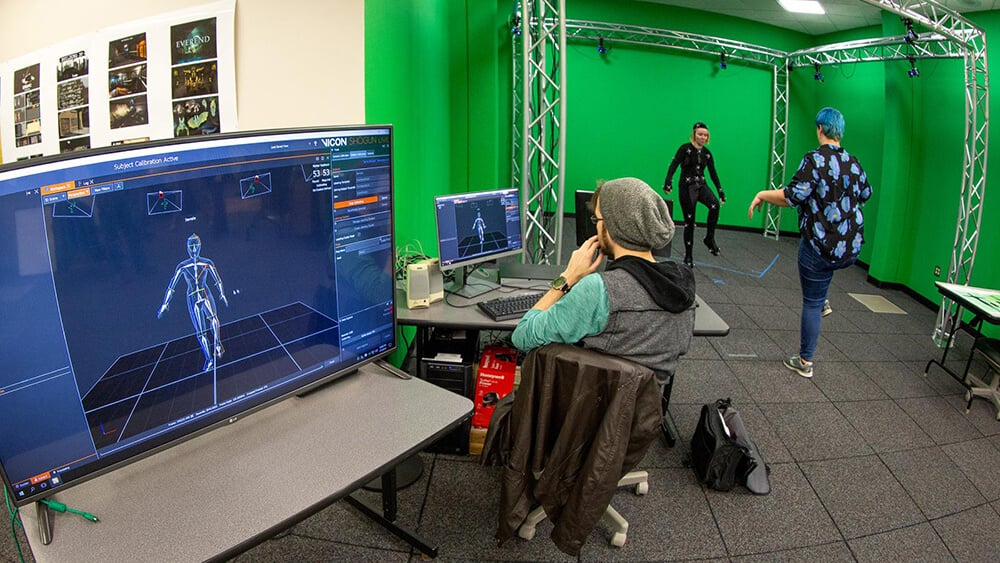
\includegraphics[width=8cm]{figure/ch2_fig_OMC_Vicon.png}
     \caption[Vicon 實驗環境與設置]{Vicon 實驗環境與設置}
     \label{ch2_fig_OMC_Vicon}
 \end{figure}

\subsubsection{無標記動作捕捉系統}
% - OpenPose、MediaPipe
    % - 看一下 OpenPose 的文獻
    % - 可在室外量測
    % - 器材架設相對容易
    % - 量測誤差約落在 7.2 公分,精準程度會隨著相機數量的減少而降低
    % - 若被遮擋,則無法辨識出被遮擋的關節
    % - 上到下或下到上的辨識(不知道找不找得到相關有提到這方面的paper)
    % - 想想看要怎麼把兩種方法的辨識結果圖片塞進去
因為光標記動作捕捉系統的限制,無標記 (marker-less) 動作捕捉系統逐漸受到重視,
其中 OpenPose ~\cite{8765346}~\cite{wei2016cpm}~\cite{simon2017hand}~\cite{cao2017realtime}、
由 Google 團隊開發的 MediaPipe ~\cite{mediapipe_web} 及由 Moicrosoft 開發的 Kinect 等系統是目前常見的無標記動作捕捉系統,
下方圖\sout{openpose mediapipe的實際應用,同一個場景,兩種辨識結果}為光標記捕捉系統的實際應用。
透過已經過校正的單一或多個攝影機同時拍攝受試者的影像,利用電腦視覺及深度學習技術辨識出受試者在二維平面上的關節點位置,
辨識關節點位置的方法分為上到下方法 (top-down method) 及下到上方法 (bottom-up method) 兩種 ~\cite{nie2019single},
上到下方法如圖 ~\ref{ch2_fig_topvsbottom} (b) 上半部分,
先辨識出受試者的周圍方塊 (detected bounding boxes),再由周圍方塊內的範圍辨識出關節點位置,例如 MediaPipe 即為上到下方法,
其缺點為若在辨識過程中找不到人,無法匡出周圍方塊,則無法辨識出關節點位置,且計算量會隨著出現在畫面中的人數增加而增加;
下到上方法如圖 ~\ref{ch2_fig_topvsbottom} (b) 下半部分,
為先偵測到關節,再將關節組成群組,最後形成特定姿勢的方法,例如 OpenPose 即為下到上方法,
其缺點為若受試者沒有完整的出現在畫面中,則有可能辨識點無法組成一個人的群組而被判斷為一個人,且也有可能會把非人類,但形狀與人類相似的關節點辨識出來。
由於最容易被大眾應用的相機為 RGB 相機,因此缺乏受試者的深度資訊,需再透過棋盤格方法相機校正及三角測量計算,取得受試者的三維姿態。 \\
% 精度
% 其量測精準度約落在\sout{ 7.2 (cm) ~\cite{8765346}},精準程度會隨著相機數量的減少而降低,adafuse
無標記動作捕捉較不受環境光限制,因此可以解決實驗場地必須設置於室內的限制,可拓展至室外進行量測,也增加了可量測的範圍及動作多樣性,
且器材架設相對容易,使用手機也可進行影像錄製,價格也相對較低,
但其缺點為易受到遮擋而影響辨識結果,若受試者的部分關節被自身遮擋或是被場域中的其他障礙物遮擋,則無法辨識出被遮擋的關節。 \\

\begin{figure}[!ht]
    \centering
    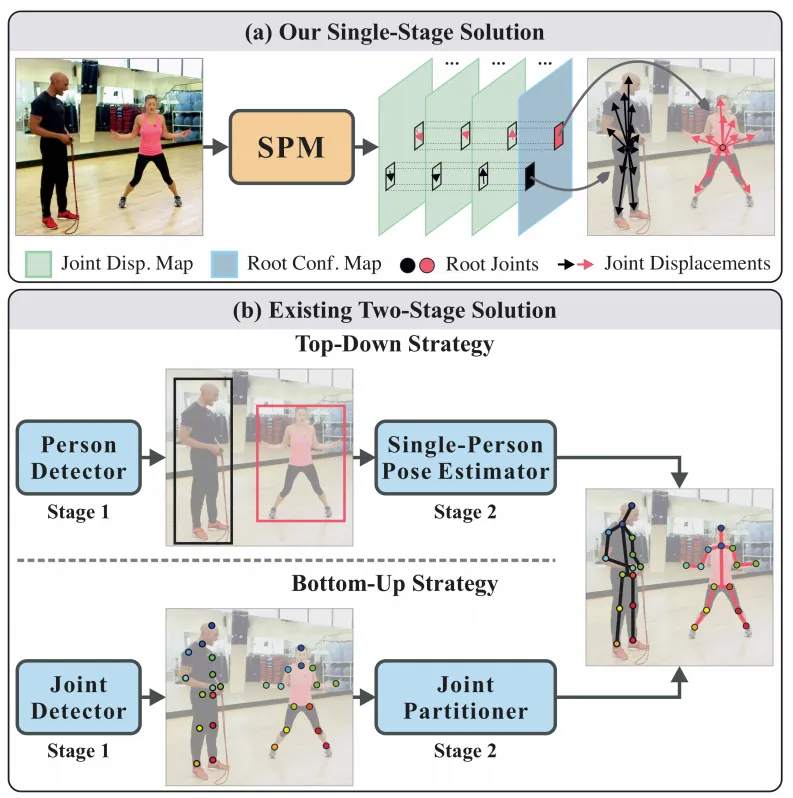
\includegraphics[width=8cm]{figure/ch2_fig_topvsbottom.png}
     \caption[辨識關節點位置的方法 ~\cite{nie2019single}]{辨識關節點位置的方法 ~\cite{nie2019single}}
     \label{ch2_fig_topvsbottom}
 \end{figure}

\subsection{單感測器-慣性動作捕捉系統}
%  - IMU
    % - 只能量測到方向,無法量測到位置
    % - 量測時常拉長後會產生 drift 的問題
以朝向為主要量測目標的慣性動作捕捉系統,則通常以慣性感測器 (Inertial Measurement Unit, IMU) 為量測工具,
一個測量單元包括加速規 (accelerometers)、陀螺儀 (gyroscopes) 及磁力計 (magnetometers),
加速規用於測量三軸加速度,陀螺儀用於測量三軸角速度,磁力計用於測量三軸磁場強度,

\subsection{多感測器動作捕捉系統}
% - 相機與 IMU 融合
% - 3DPW、totalcapture、real-time full-body…、wearable fusing…
123123

% ------------------------- 2.2 ------------------------- %
\section{個人化骨架}
個人化骨架,還沒頭緒要寫什麼
- 可能可以提及前人的做法,例如使用 Vicon 作為骨架,但是這樣的骨架不夠個人化,所以我要做這些事情

% ------------------------- 2.3 ------------------------- %
\section{時間對齊}
還沒頭緒要寫什麼
- 可能可以提及前人的做法,別人怎麼對齊的等等

% ------------------------- 2.4 ------------------------- %
\section{小結}
描述目前文獻不足的地方,所以我要做這些事情
我的部分可能就是描述目前使用的文獻都是使用 Vicon 作為骨架,我想要改善這一點,還有資料對其的地方,要再思考這不分要如何在前面2.3的章節先提到,而且可以承接章節2.2

- 骨架
- 時間對齊

% 章節回顧;個人化模型必要
本章節回顧了與研究主題相關的論文,首先從最基礎的量測技術開始介紹,
像是動作捕捉系統、力感測裝置與 EMG 等常見的量測方法,這些儀器能夠量化人體的動作表現,
透過數據處理針對特定主題來深入探討,亦可作為模擬的輸入或是輸出的驗證比較,其中量測的精準度將對應用有大幅影響,
因此在校正量測結果或是提高估計準確度上皆是重要的議題;接續介紹關於人體動作模擬的工作流程、系統、模型,
以及相關的研究文獻,研究探討不再僅限於臨床實驗當中,另外像是肌肉力量、關節扭矩等這些難以量測的資訊,
皆可在電腦中快速地取得,獲取資訊的種類增加意味著能探討的問題更加多元,大幅增廣在生物力學上的觀點;
最後針對個人化模型議題進行更深入的調查,模型準確度代表著與受試者是否有密切關聯,若僅透過通用模型進行研究,
模擬結果將與實際情況有所落差,而個人化模型能對所感興趣的資訊更真實的呈現 \cite{akhundov2022subject},
因此根據不同受試者來建立對應的個人化模型是必要的。

% 重述困境;誤差是否可接受;肌肉代償;參數抗衡
個人化模型的建立將會複雜許多,以肌肉參數為例,除了參數取得不易外,還有可能會發生肌肉代償問題 \cite{xiao2010sensitivity},
而在同一條肌肉的參數間,其亦具有參數不可識別性 \cite{bujalski2018monte},在運動軌跡預測作為驗證的文獻中 \cite{hinson2022sensitivity},
於比較軌跡的圖形裡 (文獻 Fig. 6),這個量級的誤差是否為可接受的?在肌肉代償與參數間會互相抗衡的情況下,
微小的誤差就會造成參數的估計錯誤,若誤差大到一定程度,其評估效果也將不及通用模型,
故在估計與驗證參數的過程是十分重要的 \cite{hicks2015my}。

% 論文重點;章節安排
本論文著重在肌肉參數的估計中,對於上述的問題進行深入探討與驗證,提出一套適用的估計參數研究方法,
並以已建立好的上肢模型作為驗證,除了進行參數估計外,也會呈現參數間抗衡的範例,來顯現該問題的重要性。

\clearpage